\documentclass[10pt]{article}
\usepackage[english]{babel}
\usepackage[parfill]{parskip}
\usepackage{float}
\usepackage{hyperref}
\usepackage{multirow}
\usepackage{xcolor}
\usepackage{todonotes}
\usepackage{amsmath}
% \usepackage[margin=.9in]{geometry}
\usepackage{array}
\usepackage{graphicx}
\usepackage{caption, subcaption}
\usepackage{enumitem}
\usepackage{tabularx}
\usepackage{lmodern}
% \usepackage[fontsize=9pt]{scrextend}
\usepackage[noend]{algorithm2e}


\setlength{\parskip}{1em}

\makeatletter
\renewcommand{\rmdefault}{\sfdefault}
% \def\subtitle#1{\gdef\@subtitle{#1}}

\def\leftHeader#1{\listadd\@leftHeader{#1}}
\def\rightHeader#1{\listadd\@rightHeader{#1}}

\def\@maketitle{
    \renewcommand{\do}[1]{##1

    }
    \begin{minipage}[t]{5cm}
        \flushleft
        \dolistloop{\@leftHeader}
    \end{minipage}
    \hfill
    \begin{minipage}[t]{5cm}
        \flushright
        \dolistloop{\@rightHeader}
    \end{minipage}
    \centering

    \vspace{0.7cm}
% \vfill
    {\huge\bfseries\@title\par}
% \vfill
    \vspace{0.7cm}
    \thispagestyle{empty}
}
\makeatother

\newcommand{\one}[1]{\colorbox{yellow}{$\displaystyle #1$}}
\newcommand{\two}[1]{\colorbox{green}{$\displaystyle #1$}}

\newcommand{\onen}[1]{\colorbox{yellow}{#1}}
\newcommand{\twon}[1]{\colorbox{green}{#1}}

\title{Fundamental project\\\LARGE Gradient-Free Policy Optimisation}
\leftHeader{Ward Gauderis}
\leftHeader{0588485}
\rightHeader{Reinforcement Learning}
\rightHeader{Faculteit Wetenschappen}
\rightHeader{Vrije Universiteit Brussel}
\leftHeader{01/06/2023}

\begin{document}
\maketitle

\section{Introduction}
Introduce problem

Objective of RL: maximize expected rewards

Policy gradient: parametric, maximize objective of reward times probability of action
gradient descent

local information: local + learning rate

gradient free: local search with perturbation
Less local optima, not sample efficient

zeroth-order optimisation

population-based optimisation: no learning rate


Introduce algorithms
\section{Literature Review}

HO + RL book

Literature review: alternative solutions

Particle swarm

simulated annealing

stochastic optimisation

genetic algorithms

\section{Methods}

\begin{algorithm}
    \KwIn{$\pi_\theta$: parametric policy}
    \KwIn{$\sigma$: standard deviation}
    \KwIn{$E$: number of evaluation episodes}
    \KwIn{$\alpha$: learning rate}
    \SetKwBlock{Loop}{Loop}{EndLoop}
    \Loop{
        sample $p \sim \mathcal{N}(\mathbf{0}, \sigma^2 I)$

        $r^+ \gets \text{evaluate}(\pi_{\theta+p}, E)$

        $r^- \gets \text{evaluate}(\pi_{\theta-p}, E)$

        $\Delta \gets \frac{r^+ - r^-}{2} p$

        $\pi_\theta \gets \pi_{\theta+\alpha\Delta}$}

    \caption{Zeroth-order optimisation}
    \label{alg:zeroth}
\end{algorithm}

\begin{algorithm}
    \KwIn{$\pi_\theta$: parametric policy}
    \KwIn{$\sigma$: standard deviation}
    \KwIn{$E$: number of evaluation episodes}
    \KwIn{$N$: population size}
    \SetKwBlock{Loop}{Loop}{EndLoop}
    \SetKwFor{RepTimes}{repeat}{times}{end}
    \Loop{
        $r_\text{max} \gets -\infty$

        \RepTimes{$N$}{
            sample $p \sim \mathcal{N}(\mathbf{0}, \sigma^2 I)$

            $r \gets \text{evaluate}(\pi_{\theta+p, E})$

            \If{$r \ge r_\text{max}$}{
                $r \gets r_\text{max}$

                $\pi_\theta \gets \pi_{\theta+p}$
            }
        }
    }
    \caption{Population-based optimisation}
    \label{alg:population}
\end{algorithm}

Both algorithms were run for 10\,000 iterations in the gym environment 'Lunar Lander' with a time limit of 500 steps per episode.
This limit was chosen to encourage the agents to learn efficient policies and avoid long simulation times while providing enough
to solve every episode. An episode is concidered to be solved by an agent when a cumulative reward above 200 is obtained.

After reasonable fine-tuning of the hyper-parameters, the following values were found to be suitable the zeroth-order method:
\begin{itemize}
    \item Standard deviation $\sigma=0.05$
    \item Number of evaluation episodes $E = 1$
\end{itemize}
In the experimental results, we investigate the influence of the number of evaluation episodes $E$ on the performance of the agent.
For the population-based method, the size of the perturbations was decreased and we will research the combined impact of the population size
$N$ and number of evaluation episodes $E$ on the results:
\begin{itemize}
    \item Standard deviation $\sigma=0.01$
\end{itemize}

\section{Results}

For readability the x-axis of the figures displays only the average cumulative reward per iteration of the
algorithm. To compare the performance of the different algorithms in terms of the total number of
evaluations used, one should 

\begin{figure}
    \centering
    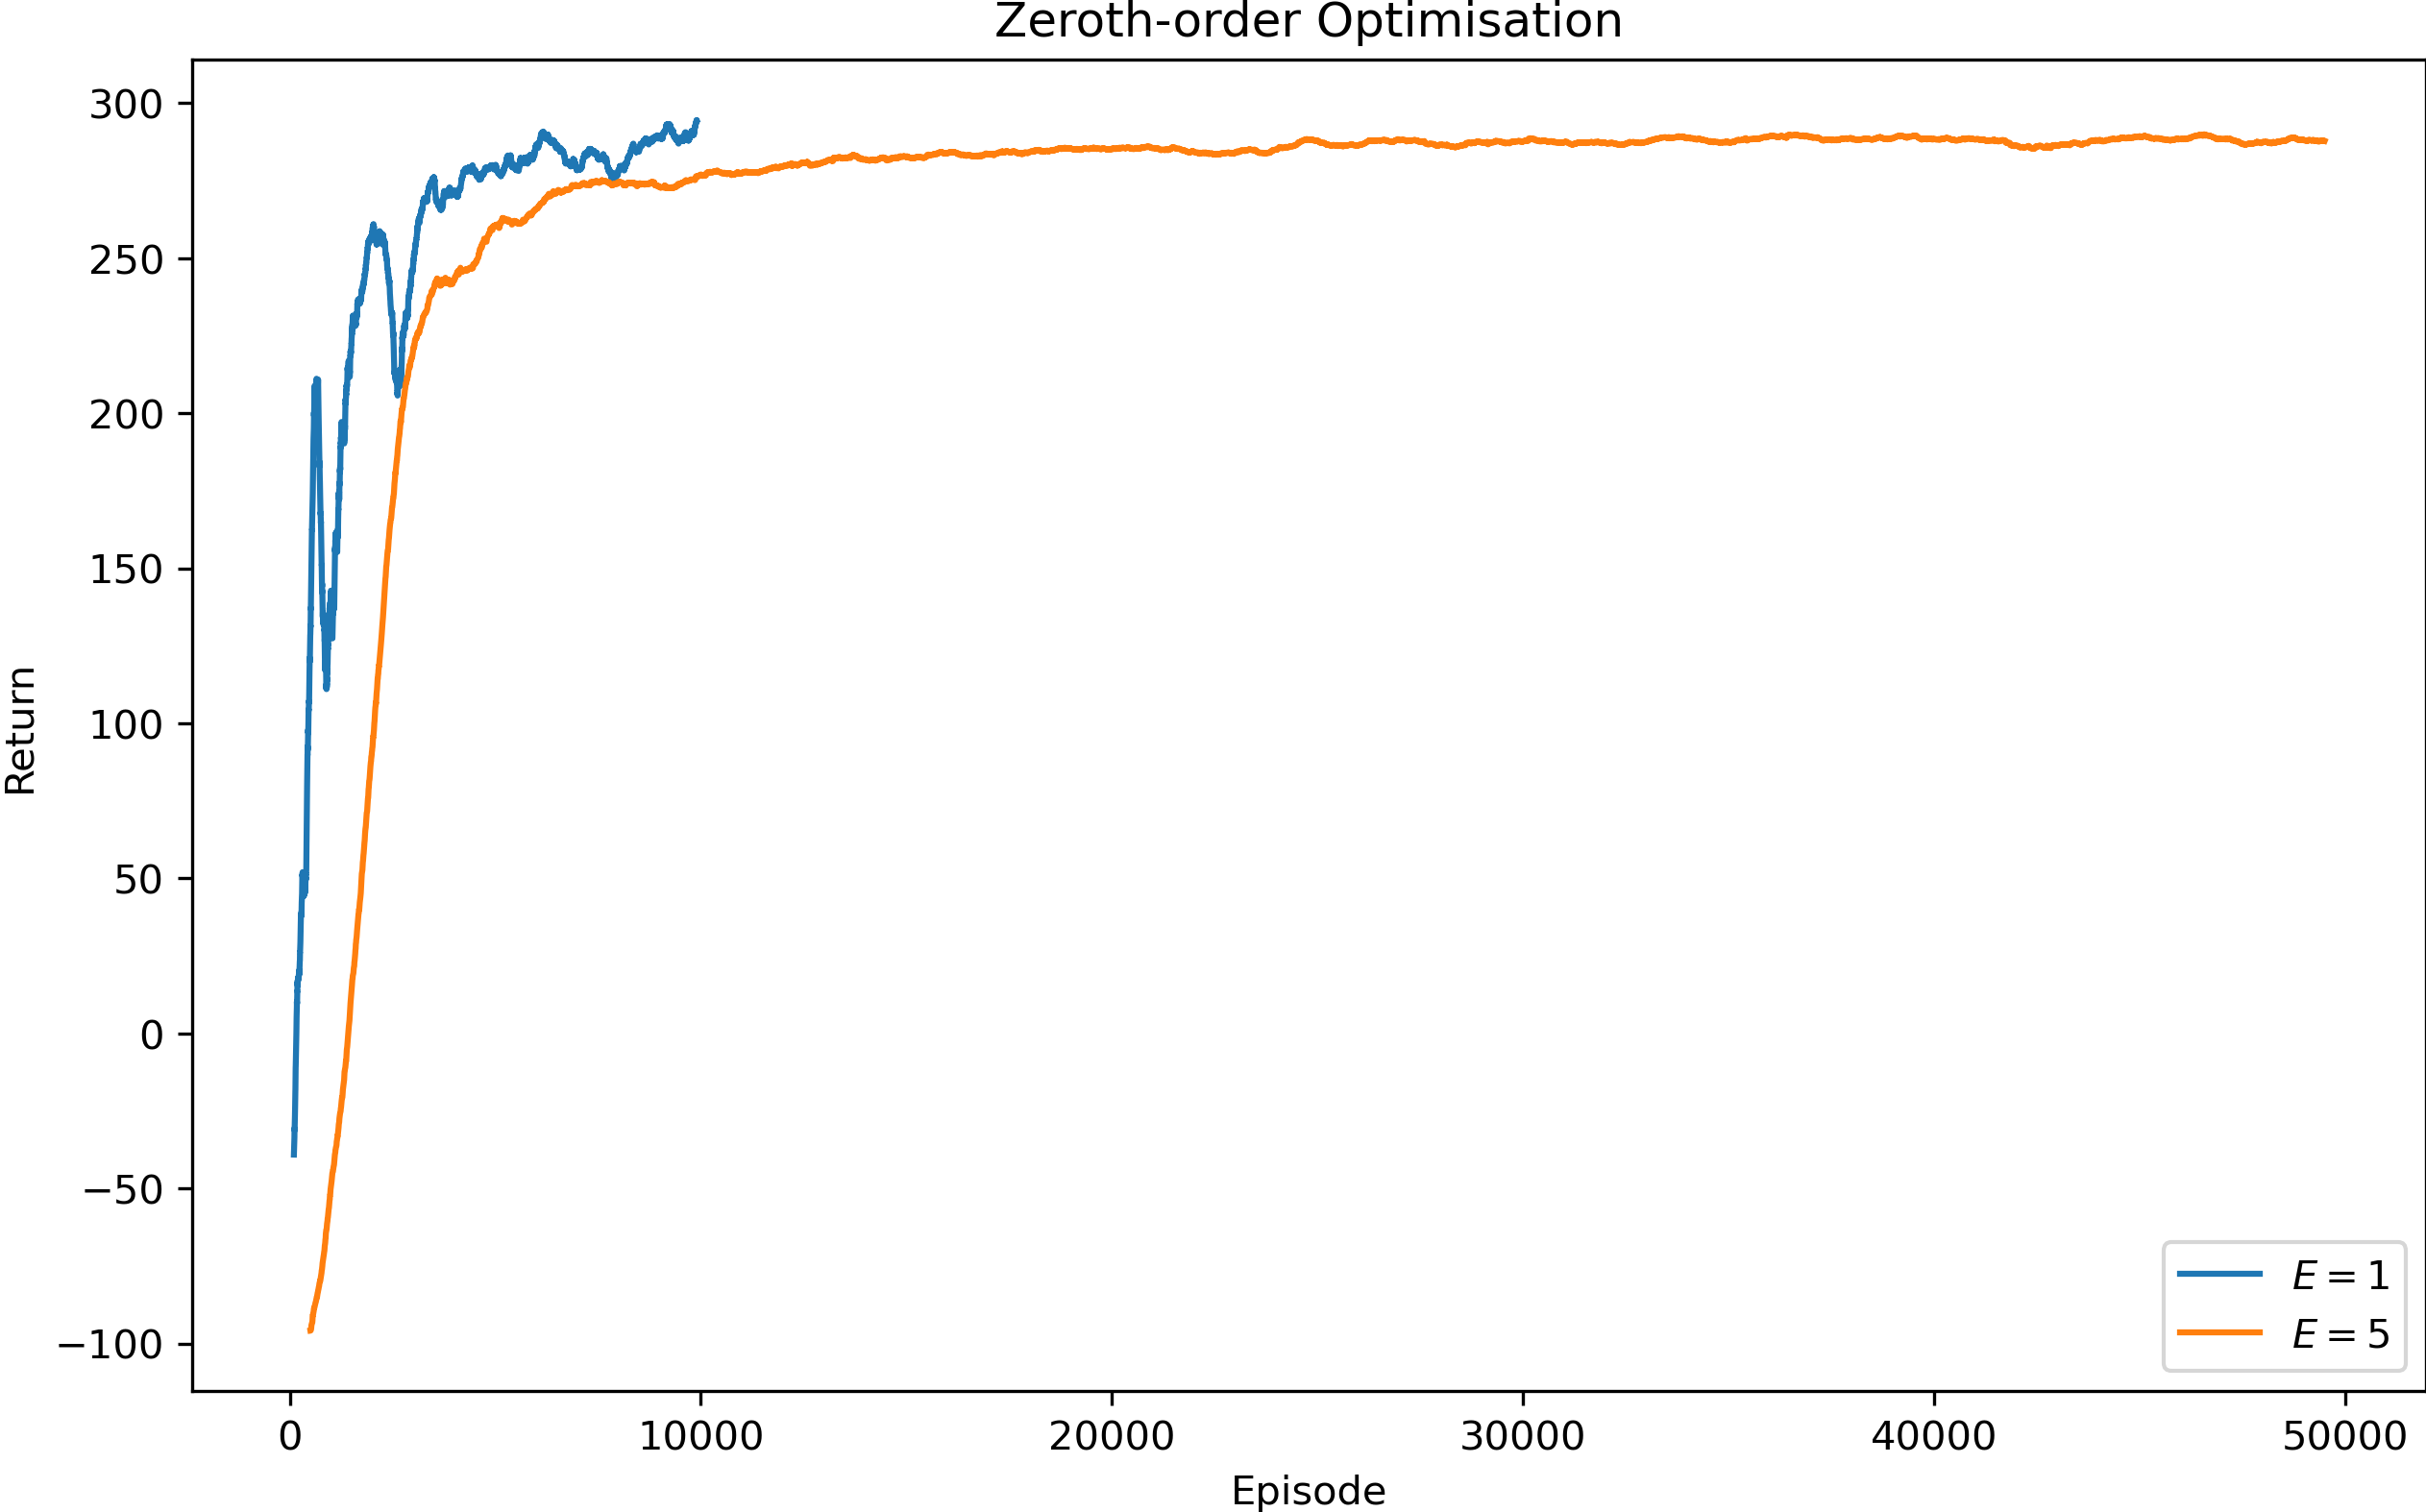
\includegraphics[width=\textwidth]{checkpoints/FINAL/zeroth_order.png}
    \caption{Cumulative reward per episode for the zeroth-order agents (averaged over 200 episodes)}
    \label{fig:zeroth_order}
\end{figure}

\begin{figure}
    \centering
    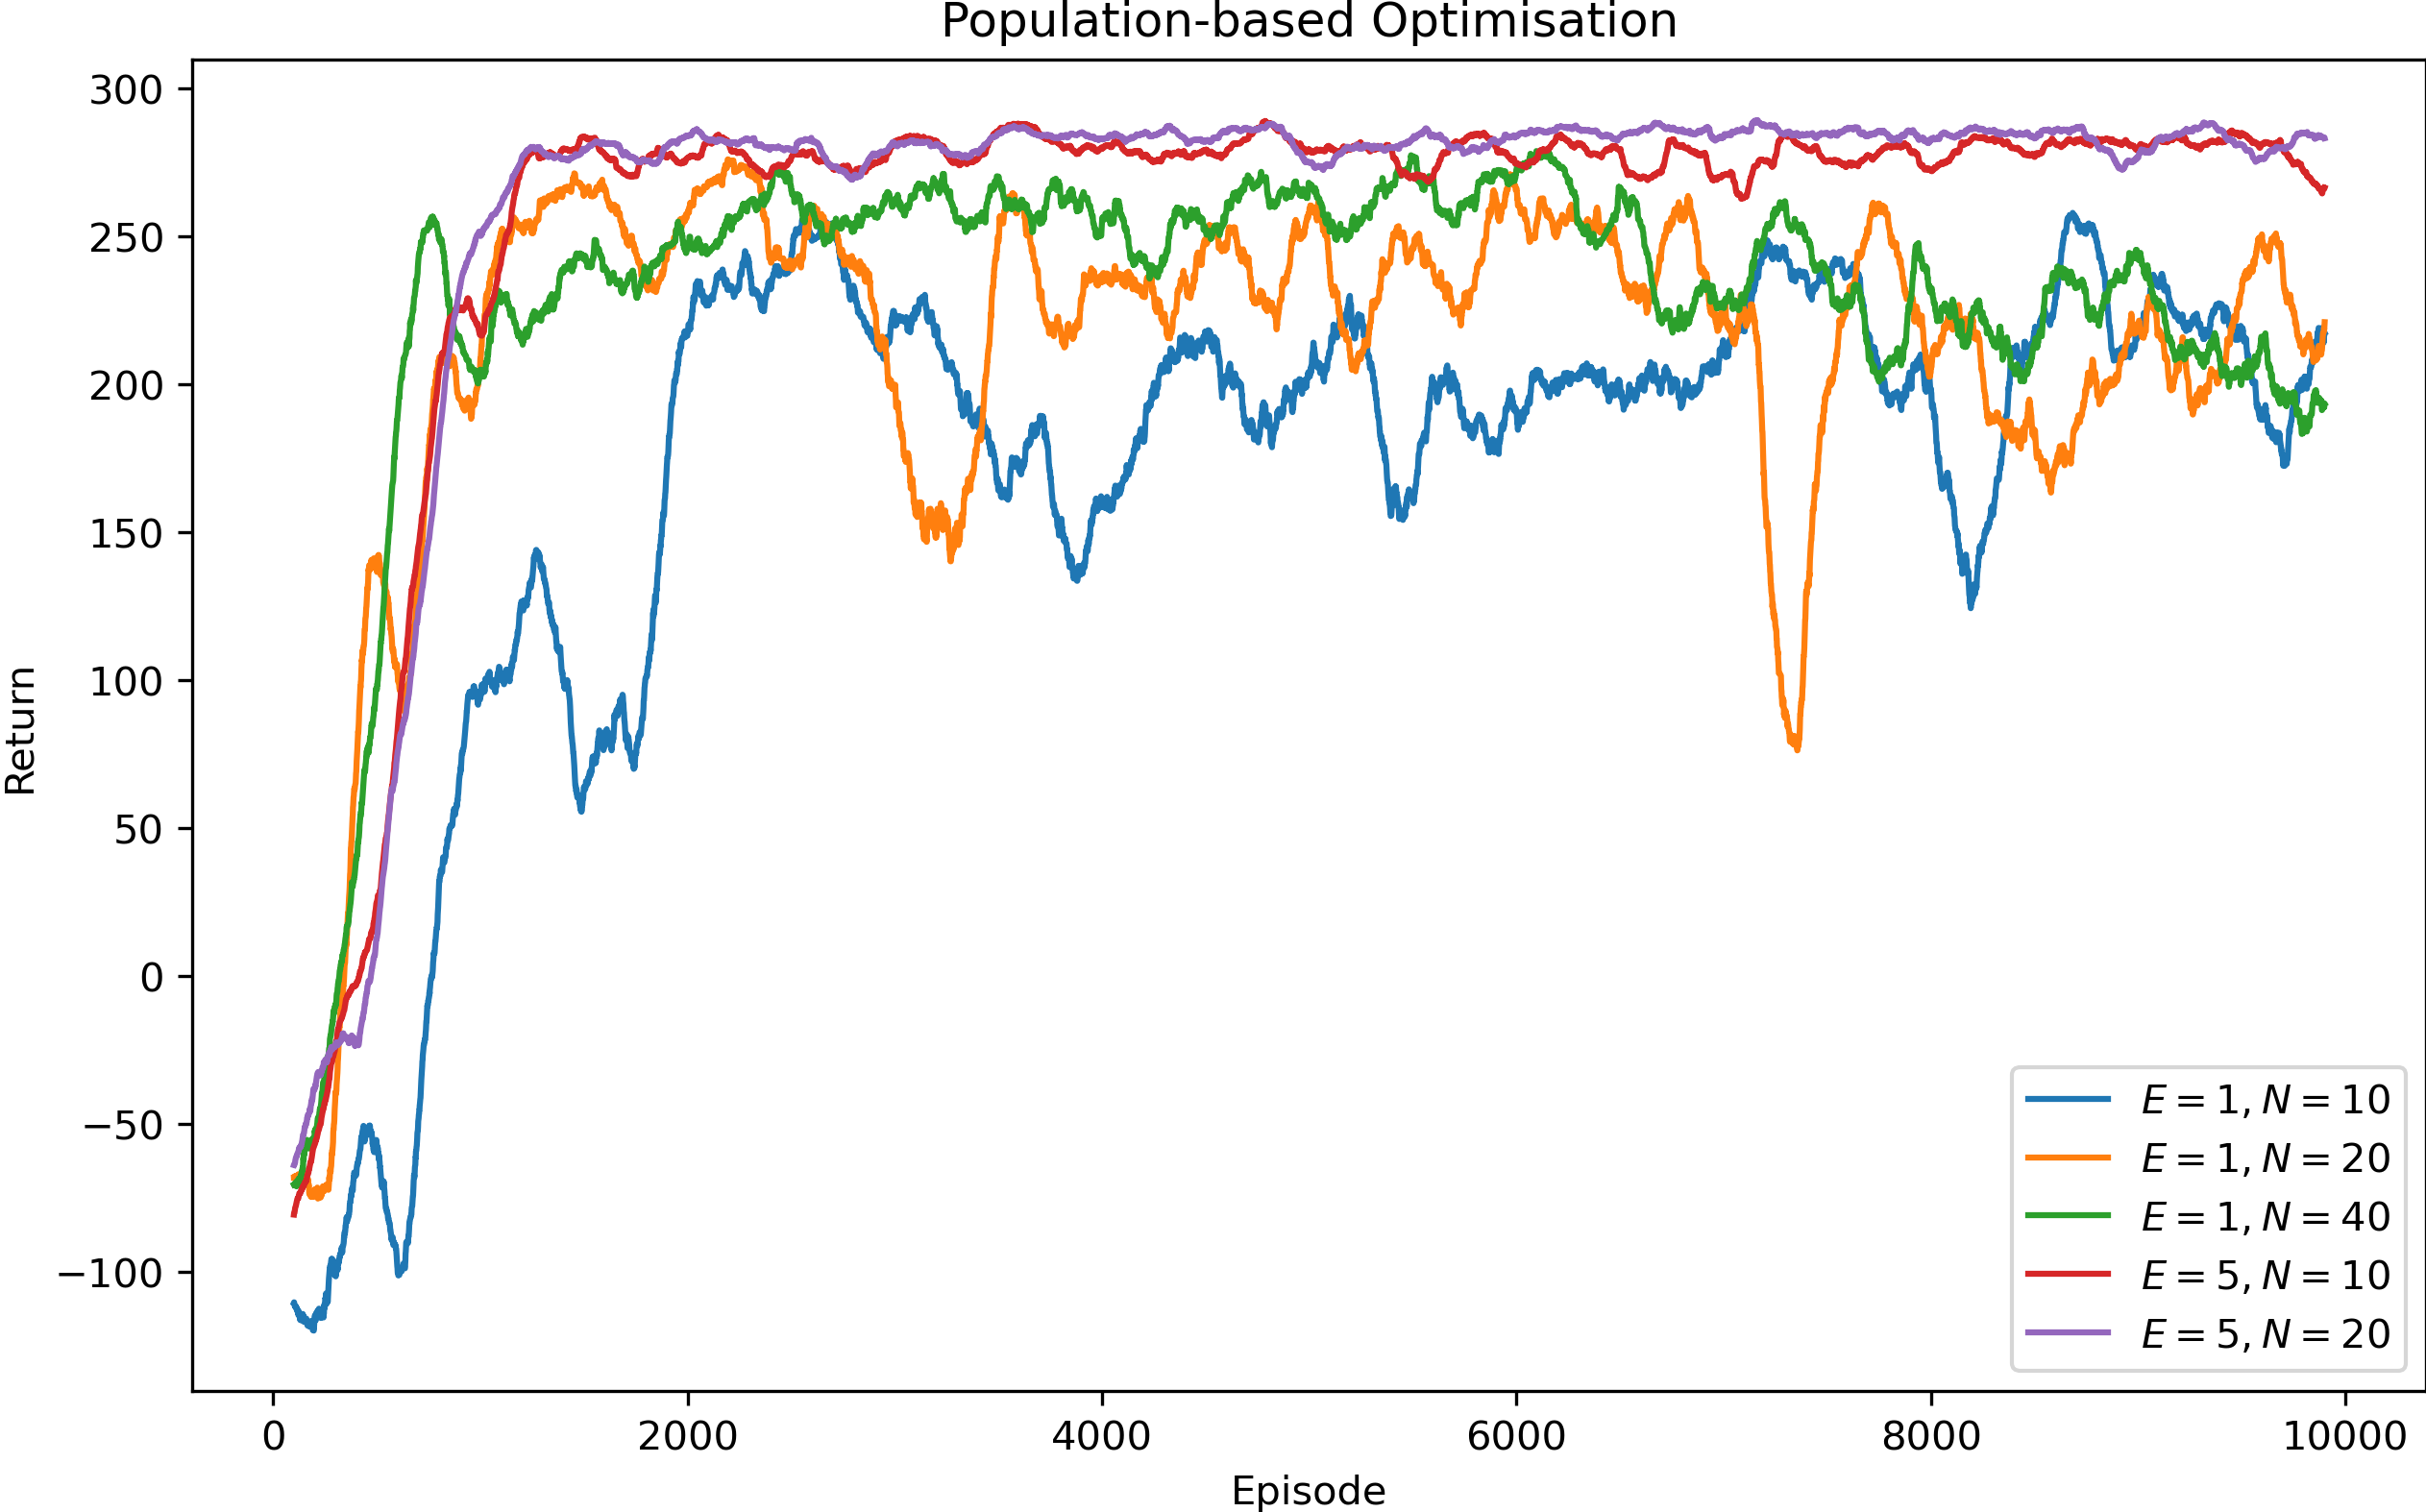
\includegraphics[width=\textwidth]{checkpoints/FINAL/population.png}
    \caption{Cumulative reward per episode for the population-based agents (averaged over 200 episodes)}
    \label{fig:population}
\end{figure}



Readability multipliplied by eval

\section{Conclusion}

% bibliography
\bibliographystyle{plain}
\bibliography{report}

\end{document}
